\documentclass[10pt,letterpaper]{article}
\usepackage[T1]{fontenc}
\usepackage[utf8]{inputenc}
\usepackage{lmodern}
\usepackage[margin=0.91in]{geometry}
\usepackage{microtype}
\usepackage{amsmath,amssymb,mathtools}
\usepackage{graphicx}
\usepackage{booktabs,tabularx,array}
\usepackage{enumitem}
\usepackage[font=small,labelfont=bf]{caption}
\usepackage{float}
\usepackage{hyperref}
\hypersetup{colorlinks=true,linkcolor=black,citecolor=black,urlcolor=blue,pdftitle={Shared Weights, Different Roles II: Mechanistic Interpretation of a Tied Loop},pdfauthor={Patrick Dugan}}
\setlength{\parindent}{1.1em}
\setlength{\parskip}{0.18em}
\setlist[itemize]{topsep=3pt,itemsep=1pt,leftmargin=*}
\renewcommand{\arraystretch}{1.14}
\newcommand{\LoopT}{\textsc{Loop-T}}
\newcommand{\FFU}{\textsc{FF-U}}
\newcommand{\EM}{\mathrm{EM}}
\newcommand{\IIA}{\mathrm{IIA}}
\newcommand{\DEF}{\mathrm{DEF}}
\newcommand{\cur}{\operatorname{cur\_node}}
\title{\bfseries Shared Weights, Different Roles II:\\[0.35em]
Mechanistic Interpretation of a Tied Loop,\\[0.15em]
from Feature Differences to Mediated Variables}
\author{Patrick Dugan}
\date{October 2026\\[0.2em]\normalsize Revised technical note; exploratory}
\begin{document}
\maketitle
\vspace{-0.7em}
\begin{abstract}
\noindent
A looped transformer reuses a block while the computational meaning of its state changes across invocations. We test whether a shared representation can survive repeated use, whether a sparse operation model can replace the block's MLP, and whether interventions recover named intermediate variables in tasks with exact reference traces. Small decoders either repeat one block eight times (\LoopT, 0.46M parameters) or use eight distinct blocks (\FFU, 1.84M). Both architectures are trained on four algorithmic task families. In three analyzed tied seeds, repeated replacement with one sparse dictionary retains 0.900--0.923 of clean deep-chain exact match; the displayed PCA comparison favors the dictionary for two seeds, while the first seed's preregistered classification requires configuration-level verification. On the analyzed untied seed, the shared dictionary retains 0.688, below matched-error PCA (0.796) and equal-norm isotropic noise (0.778). A position-local whole-block transcoder fails as a replacement, while MLP-only transcoders with native attention retained preserve 0.94--0.996 of clean deep accuracy across nine models. Sparse dictionary features satisfy the stated mediation criterion for 63\%, 91\%, and 78\% of effect-bearing transition classes in the tied seeds; the reported median selected-set sizes are four to eight features. Query-block interventions transfer an early pointer-chase node in five of six tied seeds, including three fresh seeds, at selected hop--visit cells; the remaining seed shows no mid-loop transfer. Final answers are accessible through rank-32 fitted interventions at the answer position. Variable-transfer results are exploratory maxima over intervention settings. In a registered follow-up on a fresh split, 32 or fewer dictionary features transfer the named node in four of five eligible tied seeds and in neither eligible untied seed. No sealed confirmatory split was used.
\end{abstract}

\section{Introduction}
Weight tying separates a parameter's identity from its computational role. The same transformer block encounters different states as a loop progresses, as in Universal Transformers and later looped-transformer architectures \cite{dehghani,giannou,li,saunshi}. A useful mechanistic account must therefore specify more than the weights. It must also explain the state presented to those weights and how the resulting update affects subsequent computation.

Our preceding manuscript analyzed two passes of a pretrained 3B model \cite{dugan1}. It applied invocation-specific parameter decomposition \cite{braun} and a shared sparse autoencoder \cite{bricken}. Its principal constraints were empirical: a second-pass dictionary at layer 22 explained $-0.18$ of held-out variance before a Muon control raised that value to $0.45$; no tested surrogate could stand in for the entire layer; and the available feature was selected for changing across passes rather than for carrying a named relation. Those observations motivated a test bed where intermediate quantities can be calculated independently of the model.

We use pointer chasing, gated pointer chasing, reachability, and $4\times4$ sudoku. In a pointer chase on a graph represented by a successor function $f$, the reference variable after $s$ hops from starting node $a$ is $\cur(s)=f^s(a)$. A gated chase introduces a latch, while reachability supplies a goal flag. These are variables in the task's reference computation; whether the trained network realizes them is the question under study.

The present experiments divide the question into three parts. Section~\ref{sec:dictionary} tests a shared dictionary in the full recurrent computation. Section~\ref{sec:transcoder} evaluates replacement of the learned operation. Sections~\ref{sec:mediation}--\ref{sec:variables} intervene on updates and named variables to locate causal uses of state. The results provide substantial evidence for reusable sparse descriptions and a more limited, position-dependent account of intermediate computation. A registered follow-up (Section~
ef{sec:next}) links dictionary features to the named node in most tied seeds.

\section{Models, protocol, and measures}\label{sec:setup}
\paragraph{Architectures and tasks.} Both model families use hidden dimension 128, four attention heads, eight computational stages, RMS-normalized states, and a 64-token input comprising an edge list, query fields including the start node and hop count, and an answer position. In \LoopT\ one learned block is invoked eight times. In \FFU\ eight blocks have separate parameters. Nominal parameter counts are 0.46M and 1.84M respectively. Task depths 1--8 occur in training; ``deep'' exact match (EM) refers to depths 5--8.

A depth curriculum was used for training. Some runs needed deep supervision, which applies an answer loss after each stage; \FFU\ also used input re-injection where needed. The performance gate $G_0$ is 0.98 EM on each of the four task families. All six trained tied seeds passed this gate, compared with three of six untied seeds. The original phase-2 analysis uses tied seeds 1--3 and untied seed 3. Fresh runs comprise tied seeds 4--6 and untied seeds 4 and 6. Training was reported as deterministic on the experimental hardware, with checkpoint hashes recorded for the runs.

\paragraph{Registered and exploratory decisions.} Decision rules were committed before their associated run; subsequent changes are designated post hoc. Registration at a later exploratory stage does not make a result a sealed confirmation of an earlier discovered effect. The MLP-only transcoders, expanded rank fits, and query-block patching were developed after initial results. Figures and numerical values in this technical note are drawn from those reported runs. Audit questions raised in revision were checked against the configuration-level records; the answers are given where each question arises.

\paragraph{Outcome measures.} Deep EM is accuracy on task instances at depths 5--8. For replacement experiments, we divide deep EM under the substitution by the same model's unmodified deep EM. Interchange intervention accuracy (IIA) is the fraction of patched cases whose output matches a specified counterfactual. These normalized measures answer different questions, and their sampling units must be kept distinct in a confirmatory analysis.

\section{A shared dictionary the loop can run on}\label{sec:dictionary}
A sparse reconstruction can match recorded residual states yet fail when returned to the network. For a loop, this matters at every visit: an error introduced at one step becomes part of the next step's input. We therefore evaluate a \emph{closed-loop} replacement by reconstructing the residual state after each of the eight visits before continuing computation. Dictionaries are TopK autoencoders \cite{gao}, with reported widths 1,024--8,192 and $k\in\{8,16,32\}$.

The preregistered comparison matches a PCA truncation to the dictionary's calibration reconstruction error. An isotropic-noise control has the dictionary reconstruction's error norm. The outcome \texttt{faithful\_state} requires that \emph{at least one} tested dictionary both retain $\geq0.90$ of clean deep EM and beat its matched PCA control. The registered strong negative, \texttt{open\_loop\_only}, requires every open-loop-adequate dictionary to fall to $\leq0.50$ of clean performance while the corresponding noise control remains $\geq0.90$.

\begin{table}[t]
\centering
\small
\begin{tabularx}{\linewidth}{@{}lccc>{\raggedright\arraybackslash}X@{}}
\toprule
Model & Dictionary & PCA & Noise & Preregistered status from displayed row \\
\midrule
\LoopT\ s1 & 0.923 & 0.926 & 0.805 & \texttt{faithful\_state} met by w2048 and w4096 ($k=32$), not this row \\
\LoopT\ s2 & 0.910 & 0.897 & 0.799 & \texttt{faithful\_state} met \\
\LoopT\ s3 & 0.900 & 0.821 & 0.769 & \texttt{faithful\_state} met at reported precision \\
\FFU\ s3 & 0.688 & 0.796 & 0.778 & Neither registered outcome shown \\
\bottomrule
\end{tabularx}
\caption{Closed-loop replacement, deep EM divided by clean deep EM. Rows show each model's best-accuracy dictionary. The registered \texttt{faithful\_state} rule is existential over the 12 tested configurations. For seed 1 the qualifying configurations are w2048 $k{=}32$ (0.9020 against PCA 0.8999) and w4096 $k{=}32$ (0.9165 against 0.9146). Both are strict improvements but by only 12 and 11 of 6{,}000 deep examples; the displayed w8192 row is below PCA.}
\label{tab:dictionary}
\end{table}

All three tied seeds reach the $0.90$ performance level, retaining 0.923, 0.910, and 0.900 of their clean scores in the displayed configurations (Table~\ref{tab:dictionary}). The displayed PCA comparator is lower for seeds 2 and 3, but slightly higher for seed 1 (0.926 versus 0.923). Seed 1 meets the registered rule only through two other configurations (Table~\ref{tab:dictionary} caption). Its strict PCA improvements are 12 and 11 examples out of 6{,}000, so seed 1 is a registered success that is practically a tie with PCA. Figure~\ref{fig:dictionary} shows the broader sweep, including tied configurations on both sides of the PCA diagonal.

The untied seed's shared dictionary retains 0.688 of clean performance, compared with 0.796 under matched PCA and 0.778 under equal-norm isotropic noise. The fact that structured reconstruction error impairs performance more than noise of the same norm is a particularly direct warning against judging a recurrent surrogate by open-loop reconstruction alone. It does not meet the registered strong-negative criterion because the noise score is below 0.90 and the displayed dictionary score exceeds 0.50. The untied comparison also imposes a single dictionary on eight independently trained layers. A fairer auditability comparison would permit per-layer dictionaries subject to a common total budget.

\begin{figure}[t]
\centering
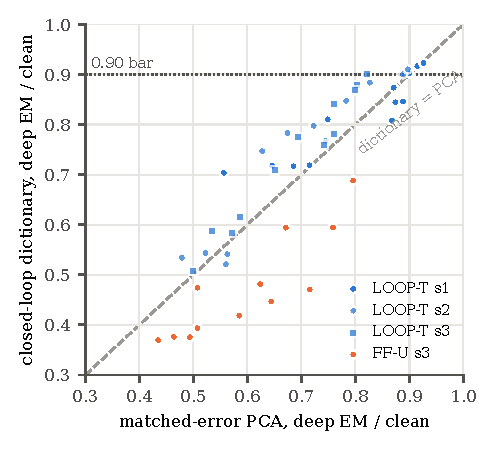
\includegraphics[width=0.49\linewidth]{figures/fig_n1_closed_loop.pdf}\hfill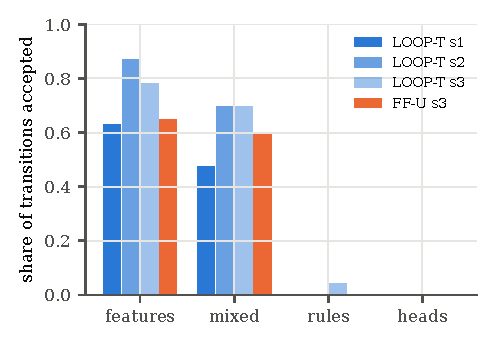
\includegraphics[width=0.49\linewidth]{figures/fig_e5_acceptance.pdf}
\caption{Left: closed-loop dictionary replacement against matched-error PCA, with 12 configurations per model; the horizontal line marks retention of 0.90 of clean deep EM. The displayed tied points lie on both sides of the PCA equality line. Right: acceptance fractions for different component bases in the update-mediation analysis of Section~\ref{sec:mediation}. Bases: \emph{features} are decoder directions of the selected shared dictionary at $t{+}1$; \emph{rules} are MLP-transcoder latent output directions at $t$; \emph{heads} are per-head output vectors; \emph{mixed} is their union ranked by raw-unit attribution.}
\label{fig:dictionary}
\end{figure}

\paragraph{Control features.} A planted direction was recovered with decoder cosine 0.84 and AUROC 0.99; an uncomputable hash bit and trace variables in randomly initialized models were not found. Features detecting particular trace variables showed 66--84\% cross-seed matches, against 2--14\% for features in general. The two visit criteria differ. A \emph{visit-index} feature is one whose activation variance across examples is at least 90\% explained by visit index; none was found. A \emph{visit-monotone} feature has a median per-example Spearman correlation of at least 0.9 between visit and activation; such features exist (Section~\ref{sec:variables}). Monotone growth within each example does not require visit index to explain most of the variance across examples.

A covariance-matched Gaussian dictionary identifies binary variables such as the latch and goal flag almost as readily as a task-trained dictionary. This limits the semantic conclusion from those detections: prominence in the state may suffice. The current-node variable is the reported exception that distinguishes task-trained dictionaries from the structure-free control. The planted-direction control should also be evaluated under the covariance-matched Gaussian baseline to establish what part of its success depends on learning task structure.

\section{Approximating the operation while keeping attention live}\label{sec:transcoder}
The registered whole-block transcoder attempted to predict each token's full update from that token's incoming state. Its residual unexplained variance plateaued at 16--27\%, and substituting it into the model reduced deep EM to approximately 0.17 of clean; predictions collapsed to a constant output. Across tested models, the attention term represented 30--42\% of update variance. Since attention depends on other token states, this creates a substantial information limitation for a position-local predictor. The observed failure is consistent with that limitation, but the experiment does not isolate attention as its exclusive cause. A whole-block surrogate allowed access to the entire sequence would test that explanation more directly.

A post-hoc alternative predicts only the MLP contribution from the MLP input, leaving the trained attention mechanism in operation \cite{dunefsky}. One MLP-only transcoder is shared over the eight visits of each tied model, while each untied layer receives its own transcoder. With width 4,096 and $k=32$, this replacement retains 0.94--0.996 of clean deep EM across the original four and five fresh models (Figure~\ref{fig:transcoder}). This tests the adequacy of a shared approximation to the MLP at the states encountered over multiple invocations.

\begin{figure}[H]
\centering
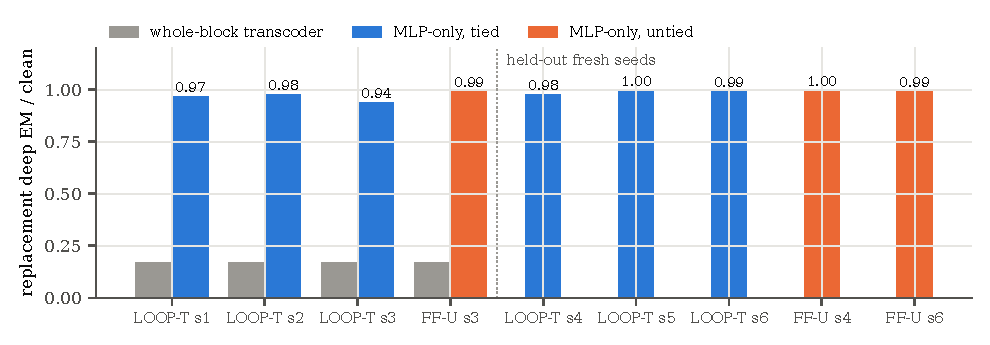
\includegraphics[width=\linewidth]{figures/fig_transcoders.pdf}
\caption{Deep EM after replacement divided by clean deep EM. Grey bars give the registered position-local whole-block transcoder on four original models. Colored bars give the post-hoc MLP-only transcoder, with attention left live, on those four models and five fresh-seed models. The figure displays individual values rounded to two decimal places.}
\label{fig:transcoder}
\end{figure}

\paragraph{Description length.} At a reported 0.95 relative-EM target, tied seeds 1 and 2 admit a single width-2,048 transcoder with approximately 1,700 active latents. The untied arm needs eight width-1{,}024, $k{=}16$ transcoders with 5{,}942 alive latents pooled across the eight (1{,}713 and 1{,}708 alive for the tied seeds). In bits, the registered count adds, per transcoder, the mean active latents per position and visit times $\log_2$ of its alive latents, plus its $128\times128$ skip matrix at 16 bits. The skip matrices dominate: 262{,}144 bits each, so the eightfold total (2.10M against 0.26M bits) largely restates the transcoder count. The latent-coding part alone is 342 against 1{,}213 bits per position and visit, about $3.5\times$. Tied seed 3 reaches only 0.947 at the tested sizes, leaving the registered description-length hypothesis unresolved.

\section{Which components restore one step's effect?}\label{sec:mediation}
For an example at visit $t$, let $r_t$ be the answer-position residual stream and $\delta$ the update at that position. We corrupt the update by replacing it with $\delta'$ from another example of the same task family and depth. A selected set of components $E$ is then restored from the difference $\delta-\delta'$. Writing $P_E$ for the restoration operator and $s(\cdot)$ for the mean log-probability assigned to the clean answer, the reported metric is
\begin{equation}
\DEF(E)=\frac{s\bigl(r_t+\delta'+P_E(\delta-\delta')\bigr)-s(r_t+\delta')}{s(\mathrm{clean})-s(r_t+\delta')}.
\label{eq:def}
\end{equation}

The denominator measures the corruption's answer-score effect. A transition class is eligible only if resampling lowers the mean clean-answer log-probability by at least 0.1 nats; this threshold was fixed in the plan before the full run. Smaller or negative effects are labelled \texttt{no\_effect} and excluded (5, 1, 1 and 4 of 24 classes for tied seeds 1--3 and the untied seed).

The acceptance rule asks whether at most 16 selected components reach $\DEF\geq0.90$ while beating five controls: random features, PCA components, MLP neurons, random directions, and orthogonal directions. Within the eligible transition classes, tied seeds 1--3 meet this rule in 63\%, 91\%, and 78\% of cases; the untied seed meets it in 65\%. Successful feature-basis reconstructions require a reported median of four to eight selected features. $S_{90}$ is the smallest $m\in\{1,2,4,8,16,32,64\}$ with $\DEF\geq0.90$ for one class; medians are over eligible classes, with classes that never reach 0.90 by $m=64$ counted as above 64 (``never''). Transcoder latents require a median of 64 components in the comparable reported analysis, and individual attention heads never satisfy the 16-component acceptance criterion (Figure~\ref{fig:dictionary}, right).

In a separate ablation, removing one of the 20 most active MLP-transcoder latents changes EM by at most 0.4--8.8 percentage points in the reported cases. Those tests give no single latent a demonstrated monopoly on an entire step. A larger deletion effect in this range deserves reporting per model; the result also leaves room for distributed or redundant representations of the step.

The component-basis comparison and the named-variable intervention are distinct tests. Recovery of a scalar answer-score effect in Equation~\ref{eq:def} does not establish that the selected features encode the reference variable $\cur(s)$. Section~
ef{sec:next} tests the link directly.

\section{Where the pointer chase is causally accessible}\label{sec:variables}
For source and base examples, an interchange intervention substitutes a source-derived state or subspace at a specified visit and token position in the base run. Its output is compared with the answer predicted by continuing on the base graph from an intermediate node of the source's reference chase \cite{geiger}. The high-level counterfactual is exactly calculable, although that does not predetermine the model's internal algorithm.

\paragraph{Answer position alone.} Early intermediate-node transfers fail under the tested full-state patches at the answer position: reported counterfactual accuracy is at most 0.22 before the final two visits. Near the end, a fitted rank-32 patch at that position transfers the final answer with IIA of 0.95--0.99, near the full-patch ceiling of 0.97--1.00 (Figure~\ref{fig:rank}). A registered rank grid ending at eight had initially produced a negative; the later expansion to higher ranks was exploratory. A \emph{doubling} abstraction, in which the state after visit $v$ holds the node $2^{v-1}$ hops from the start, scored at most 0.08 in every cell. A successful rank-32 intervention provides an upper bound on the size of the fitted intervention under its own parameterization. It does not establish a minimum intrinsic representational dimension.

\paragraph{Query-plus-answer block.} Post-hoc interventions patch four query positions along with the answer position, keeping source and base hop counts equal. At selected early-hop cells, original tied seeds 1 and 3 attain IIA of 0.68 and 0.77; fresh tied seeds 4--6 attain 0.93--1.00. Tied seed 2 shows no comparable mid-loop transfer. Two untied seeds attain 0.69 and 0.83. Later intermediate hops transfer incompletely, with reported values of 0.35--0.58. A control evaluating the source's complete final answer remains low at the relevant early cells (reported $\leq0.12$), while Figure~\ref{fig:hop} shows that this control rises when the answer forms at late visits.

\begin{figure}[t]
\centering
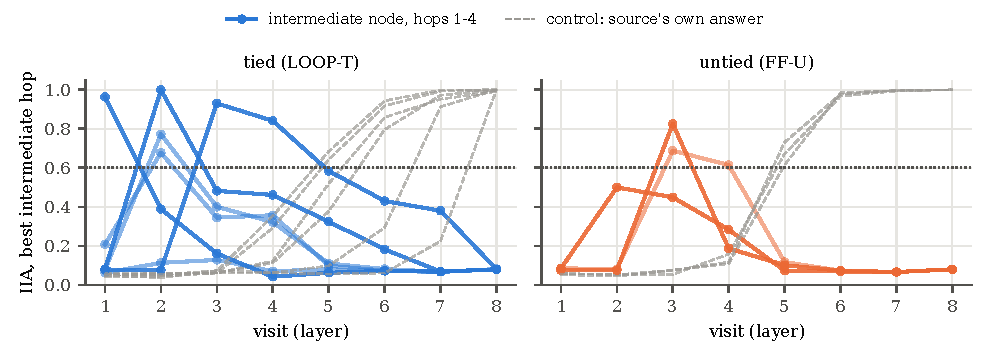
\includegraphics[width=\linewidth]{figures/fig_query_patch_schedule.pdf}
\caption{Query-block interchange interventions on pointer chasing. At each visit, each seed's solid curve shows the \emph{maximum} IIA over candidate intermediate hops 1--4. Thus the plotted curves already select over hops; the single per-seed headline values additionally select the best visit. Dashed curves score transfer of the source's completed answer. Fresh seeds are indicated by darker traces. The threshold line is at IIA 0.60. These are exploratory, maximum-selected summaries rather than fixed-cell confirmation.}
\label{fig:hop}
\end{figure}

The fresh seeds produce larger peak early-hop scores than the two original tied seeds with transfer. This could reflect differences among trained solutions or the max-selection procedure; no explanation is established by the supplied results. Table~\ref{tab:collision} gives each model's winning cell; 64 cells (8 visits by 8 hops) were tested per model and family. A confirmatory report should fix the cell before evaluating a sealed split. The failure in seed 2 must remain visible alongside the five positive tied seeds.

\paragraph{Rank and patch scope.} At the best mid-loop query-block cells, rank eight transfers little of the early node, while ranks 32--128 approach portions of the full patch's effect (Figure~\ref{fig:rank}). The plotted rank grid is $\{1,2,4,8,16,32,128\}$, omitting 64. For the query block, rank refers to one subspace of the concatenated five-position state ($5\times128=640$ dimensions), not separate per-position projections. The block patch likewise cannot localize the effect to a particular query position. Single-position and subset patches would determine which token positions are necessary.

\begin{figure}[t]
\centering
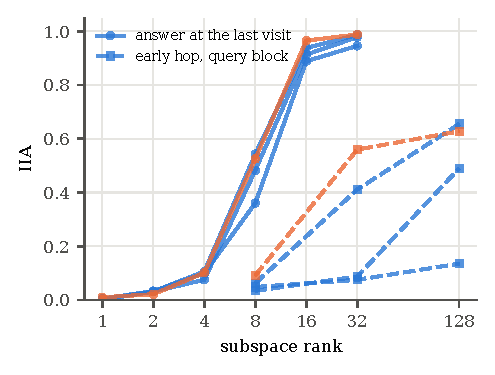
\includegraphics[width=0.72\linewidth]{figures/fig_rank.pdf}
\caption{Interchange accuracy versus fitted subspace rank for original models. Solid lines: final-answer transfer at the answer position in the last visit. Dashed lines: early-node transfer at each model's best mid-loop query-block cell. The early-node traces inherit selection over hop and visit. The plotted grid jumps from rank 32 to 128.}
\label{fig:rank}
\end{figure}

\paragraph{Discriminating an intermediate node from query copying.} Because the four query positions include the source's start node, a query-block patch may copy more than the intended intermediate variable. Let $f_B$ and $f_S$ be the base and source successor maps, $a_S$ the source start, $K$ the common requested hop count, and $s$ the intervened intermediate step. A transfer of $\cur_S(s)$ predicts
\begin{equation}
 y_{\mathrm{node}}=f_B^{K-s}\bigl(f_S^s(a_S)\bigr),\qquad
 y_{\mathrm{start}}=f_B^K(a_S)
 \label{eq:counterfactuals}
\end{equation}
for the intended node-transfer and the competing start-copy-and-recompute explanation, respectively. For $s=1$ their outputs coincide exactly when
\begin{equation}
 f_B^{K-1}\bigl(f_S(a_S)\bigr)=f_B^{K-1}\bigl(f_B(a_S)\bigr).
 \label{eq:collision}
\end{equation}
The task generator samples $f_B$ as a permutation, so it is injective and Equation~\ref{eq:collision} reduces to equality of the first outgoing edges. We regenerated the exact evaluation pairs at each model's best early-hop cell (Table~\ref{tab:collision}). Collisions occur in 5.2--6.9\% of pairs, and IIA on the non-colliding pairs is within 0.03 of the full rate. The model outputs $y_{\mathrm{start}}$ on at most 4.5\% of non-colliding pairs, with one exception: untied seed 4 does so on 49\%. Its 0.50 headline is therefore start copying, not node transfer, and it is not counted as a transfer.


\begin{table}[t]
\centering\small
\begin{tabular}{lcccccc}
\toprule
Model & Cell (visit, hop) & Pairs & Collision & IIA, all & IIA, non-colliding & Start copy \\
\midrule
\LoopT\ s1 & 2, 1 & 1000 & 0.052 & 0.677 & 0.673 & 0.027 \\
\LoopT\ s2 & 2, 1 & 1000 & 0.052 & 0.113 & 0.113 & 0.045 \\
\LoopT\ s3 & 2, 1 & 1000 & 0.052 & 0.772 & 0.772 & 0.014 \\
\LoopT\ s4 & 1, 1 & 1000 & 0.063 & 0.963 & 0.961 & 0.005 \\
\LoopT\ s5 & 2, 1 & 1000 & 0.052 & 0.999 & 0.999 & 0.000 \\
\LoopT\ s6 & 3, 1 & 1000 & 0.069 & 0.930 & 0.928 & 0.003 \\
\FFU\ s3 & 3, 1 & 1000 & 0.069 & 0.688 & 0.689 & 0.026 \\
\FFU\ s4 & 2, 1 & 1000 & 0.052 & 0.500 & 0.473 & 0.495 \\
\FFU\ s6 & 3, 1 & 1000 & 0.069 & 0.825 & 0.821 & 0.011 \\
\bottomrule
\end{tabular}
\caption{Start-copy audit of the query-block patch at each model's best early-hop cell (hop 1 or 2, source-answer control at most 0.2), with the exact evaluation pairs regenerated. Collision is the share of pairs with $y_{\mathrm{node}}=y_{\mathrm{start}}$. Start copy is the share of non-colliding pairs on which the model outputs $y_{\mathrm{start}}$.}
\label{tab:collision}
\end{table}

\paragraph{Counters and patch validity.} Visit-monotone features were found in two of the three tied seeds. Clamping one such feature to its value two visits earlier changed at most 0.6\% of answers, far below a preregistered 50\% bar. The experiment does not identify a causally used counter under that specific single-feature clamp. The study applied a norm guard to its subspace interventions, but deferred the probe-decodability guard discussed in the subspace-patching literature \cite{makelov}. Downstream checks remain necessary to distinguish faithful variable transfer from a patch that reaches the intended answer through an alternative path.

\section{What the experiments support}\label{sec:discussion}
The strongest recurrent-state result is operational: one tied dictionary preserves substantial accuracy when its reconstruction is repeatedly fed back through eight invocations. Its failure on the tested untied model is informative about sharing a basis across layers, with the architecture comparison still confounded by training success and by the different demands placed on the untied dictionary. The MLP-only transcoder result independently shows that a single operation surrogate can remain useful across different visits while the model's own attention remains active.

The mediation analysis identifies small feature sets sufficient to recover a substantial fraction of particular answer-score effects. Interchange experiments find that named pointer-chase variables can sometimes be transferred by changing a limited token block at particular visits. The registered follow-up connects them partly: in four of five eligible tied seeds a few dozen dictionary features transfer the named node, while in the untied models they do not. The features were ranked by code difference, not taken from the DEF sets, so the integrated, feature-level mechanism is supported for the dictionary but not yet for the mediation sets.

A further distinction concerns accessibility. Linear probes at the answer position can reportedly decode early nodes with scores of 0.76--1.00, although the tested early answer-position patches do not transfer those nodes. This demonstrates that decodability does not guarantee the corresponding causal intervention works at that location. It suggests that a monitoring study should specify both the variable it decodes and the effect of changing that variable using a validated intervention.

\paragraph{Limitations.} The tasks and networks are small; the algorithmic traces are exact but do not certify the network's internal implementation. The tied arm passed the training gate in six of six runs, compared with three of six untied runs. Several analyses, including query-block patching and expanded rank fits, were selected after earlier results. Some headline values maximize over a grid of 64 cells per model and have not been evaluated at frozen cells on a sealed split. One tied seed shows no early-hop transfer, and one untied seed's transfer is start copying. The results therefore remain exploratory.

\section{Registered successor experiment: do features carry the named variable?}\label{sec:next}
The rules were registered on 31 October 2026, before any run (the E5/E6 plan, ``Successor experiment''). The test uses \texttt{pointer\_chase} in a split no query-block analysis had touched, chooses the cell and ranks features on its selection half, and reports on the other half. Bases have depth 5--8, pairs share a hop count, and pairs whose counterfactual equals the base answer or whose node-transfer answer equals the start-copy answer are excluded. Features of each model's selected \texttt{D-shared} dictionary are ranked by the mean absolute source-minus-base code difference over the five block positions; the top $m$ code differences are added back through their decoder directions at the base state's scale. Controls are $m$ random alive features, the all-features patch (the reconstruction difference) and the full-block patch.

Table~\ref{tab:featlink} gives the results. Seven of nine models are eligible. Four of five eligible tied seeds are linked: at $m\le 32$, selected features recover 0.90--1.00 of the full-block transfer while random features reach at most 0.12 IIA. Neither eligible untied model is linked; their selected features recover 0.38 and 0.45 of the full block at $m=32$. \LoopT{} s3 is the tied exception: its transfer needs about 64 features. For linked models the all-features patch matches the full block, so the dictionary carries the variable that the block patch moves, and a few dozen features suffice.

The arm difference carries a confound: the untied models' selected dictionaries are four and eight times wider, so 32 features are a smaller share of the code. The feature ranking also differs from the resample-and-restore selection in Section~\ref{sec:mediation}, so this links dictionary features to $\cur(s)$ rather than linking the DEF sets themselves. With two eligible untied models the comparison is suggestive, not established.

\begin{table}[t]
\centering
\small
\begin{tabular}{lllccccc}
\toprule
Model & Dictionary & Cell & Full & All feat. & $m{=}16$ & $m{=}32$ & Verdict\\
\midrule
\LoopT{} s1 & w1024 k16 & v2, s1 & 0.670 & 0.640 & 0.405 / 0.003 & 0.605 / 0.003 & linked\\
\LoopT{} s2 & w1024 k8 & v2, s2 & 0.131 & 0.111 & 0.031 / 0.000 & 0.086 / 0.000 & ineligible\\
\LoopT{} s3 & w1024 k16 & v2, s1 & 0.773 & 0.719 & 0.008 / 0.000 & 0.215 / 0.001 & not linked\\
\LoopT{} s4 & w1024 k16 & v1, s1 & 0.968 & 0.976 & 0.427 / 0.119 & 0.942 / 0.000 & linked\\
\LoopT{} s5 & w1024 k8 & v2, s1 & 1.000 & 1.000 & 1.000 / 0.000 & 1.000 / 0.021 & linked\\
\LoopT{} s6 & w1024 k8 & v3, s1 & 0.938 & 0.939 & 0.938 / 0.048 & 0.939 / 0.104 & linked\\
\FFU{} s3 & w8192 k32 & v3, s1 & 0.733 & 0.722 & 0.178 / 0.000 & 0.277 / 0.000 & not linked\\
\FFU{} s4 & w1024 k8 & v2, s1 & 0.459 & 0.509 & 0.310 / 0.000 & 0.488 / 0.006 & ineligible\\
\FFU{} s6 & w4096 k8 & v3, s1 & 0.860 & 0.814 & 0.176 / 0.000 & 0.386 / 0.012 & not linked\\
\bottomrule
\end{tabular}
\caption{Feature-level transfer of the named node $\cur(s)$ (registered successor experiment). Reporting-half IIA on 1,000 collision-free pairs per model at the cell chosen on the selection half (visit, hop step). Feature columns give selected / random alive features. Eligible: full-block IIA $\ge 0.6$. Linked: at some $m\le 32$, selected $\ge 0.5\times$ full and selected $-$ random $\ge 0.20$. At $m=64$, \LoopT{} s3 reaches 0.652 and \FFU{} s6 0.565, outside the registered range.}
\label{tab:featlink}
\end{table}
\paragraph{Further work.} A confirmatory version should freeze a dictionary, feature-selection rule, named intermediate variable, hop, visit, and token positions on development data. Use new whole-graph or whole-seed evaluation units to avoid treating repeated probes of one graph as independent cases. For each source--base pair, compute the node-transfer and start-copy answers in advance and report the collision rate as well as accuracy where those answers differ.

It should also intervene with the feature sets selected by the resample-and-restore analysis. The principal endpoint is IIA for the named $\cur(s)$ counterfactual, compared with the full-state patch, equal-size random or PCA directions, and the original DEF restoration score. Donors reaching the same intermediate node through different prefixes would test whether transfer follows the named variable rather than incidental query content. A separate token-subset analysis can locate where the necessary information resides.

Finally, evaluate per-layer untied dictionaries under a matched total representation budget, including all gate-passing untied seeds, as a separate architecture comparison. These tests should report raw numerators and denominators, uncertainty by independent evaluation unit, and the exact selected configurations. A sealed split would turn the current exploratory claims into falsifiable, registered predictions.

\paragraph{Reproducibility and status.} The original source identifies the \texttt{rmp-v0-phase2} branch and the plot-generating entry point \texttt{research\_gym.scripts.report\_rmp\_paper\_figures}, along with experiment plans, result JSON, and checkpoint reports. The four audit items raised in revision were checked against the branch records on 31 October 2026: the seed-1 classification (\texttt{n1.json}), the eligibility threshold and $S_{90}$ definition (the E5 plan and \texttt{rmp\_phase2\_e5.py}), the description-length accounting (\texttt{h3.json}), and the collision rates (\texttt{query\_collision.json}, from \texttt{rmp\_phase2\_query\_collision.py}).

\begin{thebibliography}{11}
\setlength{\itemsep}{1pt}
\bibitem{braun} D. Braun, L. Bushnaq, S. Heimersheim, J. Mendel, and L. Sharkey. Interpretability in parameter space: Minimizing mechanistic description length with attribution-based parameter decomposition. 2025.
\bibitem{bricken} T. Bricken et al. Towards monosemanticity: Decomposing language models with dictionary learning. \emph{Transformer Circuits Thread}, 2023. \url{https://transformer-circuits.pub/2023/monosemantic-features/index.html}.
\bibitem{dehghani} M. Dehghani, S. Gouws, O. Vinyals, J. Uszkoreit, and \L{}. Kaiser. Universal transformers. \emph{ICLR}, 2019.
\bibitem{dugan1} P. Dugan. Shared weights, different roles: Mechanistic interpretation across transformer passes. Research manuscript, version 3, 9 September 2026.
\bibitem{dunefsky} J. Dunefsky, P. Chlenski, and N. Nanda. Transcoders find interpretable LLM feature circuits. \emph{NeurIPS} 37, 2024.
\bibitem{gao} L. Gao et al. Scaling and evaluating sparse autoencoders. \emph{ICLR}, 2025.
\bibitem{geiger} A. Geiger, Z. Wu, C. Potts, T. Icard, and N. D. Goodman. Finding alignments between interpretable causal variables and distributed neural representations. \emph{Conference on Causal Learning and Reasoning}, 2024.
\bibitem{giannou} A. Giannou et al. Looped transformers as programmable computers. \emph{ICML}, 2023.
\bibitem{li} S. Li, Y. Zhang, J. Guo, Q. Gu, and M. Wang. DeepLoop: Depth scaling for looped transformers. 2026.
\bibitem{makelov} A. Makelov, G. Lange, A. Geiger, and N. Nanda. Is this the subspace you are looking for? An interpretability illusion for subspace activation patching. \emph{ICLR}, 2024.
\bibitem{saunshi} N. Saunshi, N. Dikkala, Z. Li, S. Kumar, and S. J. Reddi. Reasoning with latent thoughts: On the power of looped transformers. \emph{ICLR}, 2025.
\end{thebibliography}
\end{document}
